\PassOptionsToPackage{unicode=true}{hyperref} % options for packages loaded elsewhere
\PassOptionsToPackage{hyphens}{url}
%
\documentclass[a4paperpaper,]{article}
\usepackage{lmodern}
\usepackage{amssymb,amsmath}
\usepackage{ifxetex,ifluatex}
\usepackage{fixltx2e} % provides \textsubscript
\ifnum 0\ifxetex 1\fi\ifluatex 1\fi=0 % if pdftex
  \usepackage[T1]{fontenc}
  \usepackage[utf8]{inputenc}
  \usepackage{textcomp} % provides euro and other symbols
\else % if luatex or xelatex
  \usepackage{unicode-math}
  \defaultfontfeatures{Ligatures=TeX,Scale=MatchLowercase}
\fi
% use upquote if available, for straight quotes in verbatim environments
\IfFileExists{upquote.sty}{\usepackage{upquote}}{}
% use microtype if available
\IfFileExists{microtype.sty}{%
\usepackage[]{microtype}
\UseMicrotypeSet[protrusion]{basicmath} % disable protrusion for tt fonts
}{}
\IfFileExists{parskip.sty}{%
\usepackage{parskip}
}{% else
\setlength{\parindent}{0pt}
\setlength{\parskip}{6pt plus 2pt minus 1pt}
}
\usepackage{hyperref}
\hypersetup{
            pdftitle={Disturbances amplify tree community responses to climate change in the temperate-boreal ecotone},
            pdfborder={0 0 0},
            breaklinks=true}
\urlstyle{same}  % don't use monospace font for urls
\usepackage[margin=1in]{geometry}
\usepackage{longtable,booktabs}
% Fix footnotes in tables (requires footnote package)
\IfFileExists{footnote.sty}{\usepackage{footnote}\makesavenoteenv{longtable}}{}
\usepackage{graphicx,grffile}
\makeatletter
\def\maxwidth{\ifdim\Gin@nat@width>\linewidth\linewidth\else\Gin@nat@width\fi}
\def\maxheight{\ifdim\Gin@nat@height>\textheight\textheight\else\Gin@nat@height\fi}
\makeatother
% Scale images if necessary, so that they will not overflow the page
% margins by default, and it is still possible to overwrite the defaults
% using explicit options in \includegraphics[width, height, ...]{}
\setkeys{Gin}{width=\maxwidth,height=\maxheight,keepaspectratio}
\setlength{\emergencystretch}{3em}  % prevent overfull lines
\providecommand{\tightlist}{%
  \setlength{\itemsep}{0pt}\setlength{\parskip}{0pt}}
\setcounter{secnumdepth}{0}
% Redefines (sub)paragraphs to behave more like sections
\ifx\paragraph\undefined\else
\let\oldparagraph\paragraph
\renewcommand{\paragraph}[1]{\oldparagraph{#1}\mbox{}}
\fi
\ifx\subparagraph\undefined\else
\let\oldsubparagraph\subparagraph
\renewcommand{\subparagraph}[1]{\oldsubparagraph{#1}\mbox{}}
\fi

% set default figure placement to htbp
\makeatletter
\def\fps@figure{htbp}
\makeatother

\usepackage{setspace}
\setstretch{1,5}
\usepackage{lineno}
\linenumbers
\raggedright

\title{Disturbances amplify tree community responses to climate change in the
temperate-boreal ecotone}
\date{}

\begin{document}
\maketitle

\textbf{Running title}: Tree community responses to climate change

\hypertarget{abstract}{%
\section{Abstract}\label{abstract}}

\textbf{Aim} Climate change causes major shifts in species
distributions, reshuffling community composition and favoring
warm-adapted species (``thermophilization''). Tree community response is
likely to be affected by major disturbances such as fire and harvest.
Here, we quantify the relative contributions of climate change and
disturbances to temporal shifts in tree composition over the last
decades and evaluate whether disturbances accelerate community
thermophilization.

\textbf{Location} Québec, Canada

\textbf{Time period} 1970-2016

\textbf{Taxa studied} Trees

\textbf{Methods} Using 6281 forest inventory plots, we quantified
temporal changes in species composition between a historical
(1970--1980) and a contemporary period (2000--2016) by measuring
temporal ß diversity, gains and losses. The effects of climate and
disturbances on temporal ß diversity were quantified using multiple
regressions and variation partitioning. We compared how community
indices of species temperature preference (CTI) and shade tolerance
(CSI) changed for forests that experienced different levels of
disturbance. We quantified the contribution of species gains and losses
to change in CTI.

\textbf{Results} Temporal ß diversity was mainly driven by disturbances,
with historical harvesting as the most important predictor. Despite the
prevailing influence of disturbances, we revealed a significant
thermophilization (\(\Delta\)CTI~=~+0.03°C/decade) throughout forests in
Québec. However, this shift in community composition was weakly
explained by climate change and considerably slower than the rate of
warming (+0.14°C/decade). Importantly, thermophilization was amplified
by moderate disturbances (+0.044°C/decade), almost a three-fold increase
compared to minor disturbances (+0.015°C/decade). The gains and losses
of a few tree species contributed to this community-level shift.

\textbf{Conclusions} Our study provides evidence that disturbances can
strongly modify tree community responses to climate change. Moderate
disturbances, such as harvesting, may reduce competition and facilitate
gains of warm-adapted species, which then accelerate thermophilization
of tree communities under climate change. Although accelerated by
disturbances, community thermophilization was driven by the gains and
losses of a small number of species, notably gains of maples.

\hypertarget{keywords}{%
\subsection{Keywords}\label{keywords}}

Beta diversity, Climate change, Community temperature index, Community
temporal change, Disturbances, Forest, Québec, Temperate-boreal ecotone,
Thermophilization.

\pagebreak

\hypertarget{introduction}{%
\section{Introduction}\label{introduction}}

Climate warming over the past century has led to distribution shifts in
many species (Parmesan \& Yohe, 2003). Despite the general trend of
poleward and upward (in altitude) range shifts, the timing, magnitude
and even direction of species shifts vary considerably among taxa and
regions (VanDerWal \emph{et al.}, 2013). Major reshuffling of community
composition is therefore expected. Yet, we lack an understanding of the
community-level consequences of climate-driven shifts. This knowledge
gap is even greater in forests where tree response is slow (Sittaro
\emph{et al.}, 2017) relative to the short duration of typical
ecological studies. So far, much of the emphasis has been placed on
detecting species shifts at their range edge, where early signs of
changes are expected to be readily detectable (Jump \emph{et al.},
2009). As such, there is a growing body of evidence for contemporary
shifts in tree species distributions along altitudinal gradients in
mountains (Beckage \emph{et al.}, 2008; Lenoir \emph{et al.}, 2008;
Savage \& Vellend, 2015), where ecotones are narrow and well-defined
(Jump \emph{et al.}, 2009). Similar evidence is also beginning to emerge
for latitudinal shifts (Fisichelli \emph{et al.}, 2014; Sittaro \emph{et
al.}, 2017; Boisvert‐Marsh \emph{et al.}, 2019). Though, because of the
focus on shifts at range limits (e.g., leading and rearing edges of
species ranges), there has been little empirical work on the effect of
climate change on tree community composition and abundance distributions
within the core of species range itself (e.g.~ Esquivel-Muelbert
\emph{et al.}, 2018; Searle \& Chen, 2017).

Worldwide increases in tree mortality rates triggered by drought and
heat stresses have been documented recently (Allen \emph{et al.}, 2010).
In the long term, even minor changes in demographic rates can modify the
balance between local species gains and losses, leading to temporal
change in community composition. Yet, as trees are long-lived species,
mortality and recruitment rates are low (Iverson \& McKenzie, 2013).
Thus, tree community responses to contemporary climate warming are
likely to be lagged, resulting in extinction debts (Svenning \& Sandel,
2013; Talluto \emph{et al.}, 2017). Consequently, tree community-level
response to climate change remains difficult to quantify and is probably
underestimated.

Furthermore, in northern temperate and boreal regions, natural
disturbances (fires and insect outbreaks) and anthropogenic disturbances
(timber harvesting) are major drivers of tree community dynamics
(Goldblum \& Rigg, 2010). These pulse disturbances are likely to
dominate local, short-term biotic changes, resulting in increased
prevalence of young forests dominated by early successional species.
These short-term effects could easily mask climate-induced changes that
are expected to occur on much longer time scales and broader spatial
scales. For this reason, disturbances are often considered to be
inconvenient confounding factors instead of an inherent part of
contemporary ecosystems. Thus, numerous studies have searched for trends
in relatively undisturbed systems (Parmesan \& Yohe, 2003) rather than
accounting for their effects. Yet, disturbances and climate change have
a high potential for interactions, which can lead to synergistic or
antagonistic ecological effects that are difficult to predict (Brook
\emph{et al.}, 2008). Indeed, disturbances create canopy openings that
could facilitate the northward migration of temperate species (Leithead
\emph{et al.}, 2010; Xu \emph{et al.}, 2012; Vanderwel \& Purves, 2014;
Boisvert‐Marsh \emph{et al.}, 2019). In addition, the frequency and
intensity of natural disturbances can increase as an indirect effect of
climate change (Seidl \emph{et al.}, 2017).

Although it is widely assumed that positive synergy between disturbances
and climate warming should play a key role in contemporary tree
community changes, empirical studies have reached conflicting
conclusions. For example, comparison of early industrial (early 1900) to
contemporary forests in the Bas-Saint-Laurent region of Québec showed
that logging practices turned old-aged conifer forests into young mixed
and deciduous forests (Boucher \emph{et al.}, 2006, 2009). Leithead
\emph{et al.} (2010) also observed that the establishment of southern
temperate species in the temperate-boreal ecotone of northern Ontario
increased with the size and age of canopy gaps. While Boisvert‐Marsh
\emph{et al.} (2019) found that climate change outweighs disturbances in
explaining latitudinal shifts of tree saplings in Québec in the last
decades, Danneyrolles \emph{et al.} (2019) found larger impacts of
anthropogenic disturbances than climate warming on forest compositional
changes in southern Québec over the last centuries. Hence, to anticipate
and adapt to future forest changes, large-scale empirical studies are
required in order to unravel individual and aggregated impacts of
multiple stressors on forest composition.

Even though disturbances may mask slow community responses to climate
change, these two drivers leave distinguishable signatures on
communities. Climate warming should favor warm-adapted species at the
expense of cold-adapted species, leading to a ``thermophilization'' of
communities (De Frenne \emph{et al.}, 2013; Savage \& Vellend, 2015).
Conversely, disturbances should increase the prevalence of young forests
dominated by shade-intolerant species (Boucher \& Grondin, 2012; Savage
\& Vellend, 2015). Hence, analyzing shifts of relevant functional traits
and ecological affinities in communities using large-scale monitoring
data should disentangle the role of different environmental drivers in
shaping communities (Violle \emph{et al.}, 2007). For instance, the
Community Temperature Index (CTI) has been used to measure
thermophilization in various communities, such as plants, trees, birds
and fishes (Devictor \emph{et al.}, 2008; Cheung \emph{et al.}, 2013; De
Frenne \emph{et al.}, 2013; Feeley \emph{et al.}, 2013; Gaüzère \emph{et
al.}, 2015; Becker‐Scarpitta \emph{et al.}, 2019; Danneyrolles \emph{et
al.}, 2019). The CTI is a community abundance-weighted average of the
Species Temperature Indices (STI; proxy for species thermal preference
computed as the mean temperature of a given species distribution).
Because CTI reflects the relative abundance of warm-adapted (high STI)
vs cold-adapted species (low STI), it is expected to increase following
climate warming if species are moving according to their temperature
requirements.

Here, we quantify the temporal shifts in tree community composition in
the temperate-boreal ecotone, and test whether recent climate change is
impacting forest composition. We analyzed data from a long-term forest
inventory program across meridional Québec, where vegetation ranges from
northern hardwood forests dominated by \emph{Acer saccharum} at low
latitudes (up to 47°N) to mixed forests dominated by \emph{Abies
balsamea} (from 47°N to 48°N), to boreal forests dominated by
\emph{Picea mariana} at high latitudes (from 49°N to 52°N). This dataset
allowed us to compare community responses to recent climate change in
plots that experienced different levels of disturbances along a broad
latitudinal gradient. We address four questions: (1) how has the
composition of forest communities changed during the last decades across
different bioclimatic domains? (2) What is the relative contribution of
climate change and disturbances to these temporal community changes? (3)
Have forest communities experienced a thermophilization during the last
decades? And can disturbances accelerate community thermophilization?
(4) How do gains and losses of specific tree species contribute to
thermophilization?

Specifically, we measured temporal ß diversity (Legendre, 2019) over
6000 resurveyed communities between a historical (1970--1980) and a
contemporary (2000--2016) period. Temporal ß diversity, which describes
the temporal dissimilarity in community composition between survey
times, was decomposed into gains and losses to investigate the
underlying mechanisms of change. Then, we quantified the effects of
climate change and disturbances on temporal ß diversity using multiple
regressions and variation partitioning. Using community indices for
temperature (CTI) and shade tolerance (CSI), we quantified
community-level changes associated with thermophilization and succession
and compared these changes among levels of disturbances. We finally
quantified the species-specific contributions to thermophilization.

\hypertarget{methods}{%
\section{Methods}\label{methods}}

\hypertarget{study-area}{%
\subsection{Study area}\label{study-area}}

To analyze large-scale temporal changes in forest community composition,
we used the Québec forest inventory plots that have been sampled in six
bioclimatic domains, south of the 52\textsuperscript{nd} parallel, since
1970 by the Ministère des forêts, de la Faune et des Parcs (Fig. 1;
MFFP, 2016). For each plot, we compared the tree composition between the
first and last surveys. To maximize the time interval between surveys,
only plots that were inventoried in two distinct time periods
(historical period: 1970--1980; contemporary period: 2000--2016) were
retained for analysis. We disregarded plots that were subjected to
active reforestation during the study period as we were interested in
compositional changes resulting from natural post-disturbance
recolonization. We also eliminated plots without trees (due to a
disturbance) either at their first or last year of sampling. This
yielded a subset of 6281 plots analyzed (Fig. 1), with a median of 35
years between surveys (1st quartile: 33 and 3rd quartile: 41 years).

Within each circular plot (400 m\textsuperscript{2}), trees larger than
9 cm in diameter at breast height (DBH) were identified to species,
measured and their vitality noted (MFFP, 2016). The selected plots
included a total of 51 tree species, from which we eliminated introduced
and planted species as well as species with a single occurrence,
yielding 45 analyzed species (Table S1). Rare species were included in
the analyses because even the rarest can contribute to temporal changes;
their identity does not bias our analyses and, contrary to mobile
species, there is little detection bias in tree surveys. Each species
was assigned according to their functional traits to one of three
species groups of interest: boreal (6 species), pioneer (9 species) and
temperate (30 species; see Table S1 for details).

\hypertarget{environmental-variables}{%
\subsection{Environmental variables}\label{environmental-variables}}

The annual past climatic conditions, covering a period from 1960 to
2013, were extracted using a 2 km\textsuperscript{2} (60 arc sec)
resolution grid for the entire study area using the ANUSPLIN climate
modeling software (http://cfs.nrcan.gc.ca/projects/3/8; McKenney
\emph{et al.}, 2011). Bioclimatic variables hypothesized to influence
tree survival were intercepted at plot locations: the mean temperature
and total precipitation during the growing season, minimum temperature
of the coldest period, maximum temperature of the warmest period and the
annual climate moisture index (CMI; difference between annual
precipitation and potential evapotranspiration). From these bioclimatic
variables, we derived different predictors (see Table 1 for details).
Over the past four decades, growing season temperature and precipitation
have increased by 0.14 °C/decade and 9.5 mm/decade, respectively, while
CMI has decreased by 1.2 cm/decade (Fig. S1).

We also collected information pertaining to natural and anthropogenic
disturbances that have affected the forest plots both before and during
the study period (Table 1, Fig. S2). At each plot, 21 disturbance types
and their level of intensity (moderate or major) were recorded (Table
S2; MFFP, 2016). The MFFP defined major disturbances as events that
resulted in a loss of at least 75\% of the tree basal area, whereas
moderate disturbances have caused between 25\% and 75\% of loss. For our
regression models, we differentiated two main types of disturbances:
natural disturbances and harvest, with 3 levels of intensity each
(minor, moderate or major) and 2 periods (old: occurred before the first
inventory, and recent: occurred during the study period). To compare
diversity measures among disturbance levels, we also assigned each
forest to the level of intensity of the worst disturbance it experienced
(regardless of the type or timing).

Core samples were also collected on selected trees during surveys to
measure their age. Stand age was estimated as the mean of these measures
to account for forest succession processes after disturbances. Finally,
because the time interval between the first and last measurements varies
among the forest plots, it was included as a predictor.

\hypertarget{analysis}{%
\subsection{Analysis}\label{analysis}}

\hypertarget{uxdf-diversity}{%
\subsubsection{ß diversity}\label{uxdf-diversity}}

For each plot, we computed temporal ß diversity (Legendre, 2019), which
is the dissimilarity in species composition between two surveys of a
given plot, by comparing local tree abundance (i.e.~number of
individuals) in forest plots between the historical (1970-1980, \(t_1\))
and contemporary (2000-2016, \(t_2\)) periods. The dissimilarity (ß) was
computed using the Ružička coefficient (Fig. S3):

\(\beta = (B+C)/(A+B+C)\) where, for \(n\) species:

\(A = \sum_{j=1}^n a_j\)~: unscaled similarity. \(a_j\) represents the
abundance of species \(j\) that is common between \(t_1\) and \(t_2\);~

\(B = \sum_{j=1}^n b_j\)~: unscaled species abundance losses. \(b_j\)
represents the abundance of species \(j\) present at \(t_1\) but not at
\(t_2\); when species \(j\) increases in abundance, \(b_j\) = 0;

\(C = \sum_{j=1}^n c_j\)~: unscaled species abundance gains. \(c_j\)
represents the abundance of species \(j\) present at \(t_2\) but not at
\(t_1\); when species \(j\) decreases in abundance, \(c_j\) = 0;

This temporal ß diversity varies from 0 (community compositions at
\(t_1\) and \(t_2\) are exactly the same) to 1 (communities have no
shared species). The use of this dissimilarity index enabled us to
decompose the compositional change into relative gains (\(C/(A+B+C)\))
and losses (\(B/(A+B+C)\)) in tree abundances (Fig. S3). Throughout this
paper, gains and losses refer to these relative metrics.

This additive framework allowed us to partition further the different
components contributing to ß diversity. Temporal dissimilarity in tree
community can be decomposed into the dissimilarity (gains and losses) of
different species groups of interest, here boreal, pioneer and temperate
species (Table S1). The temporal dissimilarity of a given group, for
instance boreal, relative to all species is simply:
\(\beta_{boreal} = (B_{boreal}+C_{boreal})/(A+B+C)\), with \((A+B+C)\)
the denominator computed over all tree species. As a consequence, ß can
be decomposed as follows:

\(\beta = \beta_{boreal} + \beta_{pioneer} + \beta_{temperate}\)

\hypertarget{assessing-the-relative-importance-of-drivers-of-community-changes}{%
\subsubsection{Assessing the relative importance of drivers of community
changes}\label{assessing-the-relative-importance-of-drivers-of-community-changes}}

We evaluated the effects of multiple drivers on temporal ß, gains and
losses using multiple regressions, in combination with variation
partitioning analyses (Borcard \emph{et al.}, 1992; Peres-Neto \emph{et
al.}, 2006). For these analyses, we used a logit transformation
\(y'=log(y/(1-y))\) of the response variables (ß, gains, losses) as they
were all in the standard unit range {[}0, 1{]}.

In order to quantify the variation explained by climate change and
disturbances, while controlling for the baseline climate gradient and
different time intervals, we classified our predictor variables into
three subsets: baseline conditions, climate change and disturbances (see
Table 1). We then generated regression models predicting ß, gains and
losses, for each of the three subsets. We also tested relevant
interactions between disturbance and climate predictors: Natural (old
and recent) \(\times\) \(\Delta\)CMI and Natural (old and recent)
\(\times\) \(\Delta\)Temp, because drought and heat stress can increase
natural disturbance frequency; Harvest (old and recent) \(\times\)
\(\Delta\)Temp), because the effect of harvest was hypothesized to be
influenced by warmer temperatures. A forward selection of explanatory
variables based on two stopping criteria (significance level \(\alpha\)
and global \(R^2_{adj}\); Blanchet \emph{et al.}, 2008) was performed to
obtain parsimonious regression models for each of the three subsets. The
predictors had been previously standardized to \emph{z}-scores to allow
comparison of their slope coefficients. We also ensured that residuals
met the assumptions of normality and homoscedasticity.

We assessed the unique contributions of each predictor subset (baseline
conditions, climate change and disturbances) as well as their shared
effect on forest community changes using variation partitioning analysis
on the parsimonious regression models.

\hypertarget{functional-index-of-community-change}{%
\subsubsection{Functional index of community
change}\label{functional-index-of-community-change}}

To test whether or not climate warming contributed to community changes,
we examined the temporal changes in the distribution of species
temperature values within every plot. We quantified such changes by the
shift in the mean (Community Temperature Index or CTI; Devictor \emph{et
al.}, 2008), as well as the lower 10\textsuperscript{th} percentile and
the upper 90th percentile of this plot-level distribution (De Frenne
\emph{et al.}, 2013).

To compute these metrics, we first combined climate and tree occurrence
data to obtain species temperature distributions. Specifically, we
overlaid interpolated climate data (mean annual temperature averages for
1970--2000 at a spatial resolution of 1 km\textsuperscript{2}, available
online http://worldclim.org/version2; Fick \& Hijmans, 2017) and
occurrence data from multiple forest inventory databases of eastern
North America (collected in the QUICC-FOR project;
https://github.com/QUICC-FOR) for the focal species. The mean annual
temperature for each occurrence was extracted to infer species
temperature distributions. Following Devictor \emph{et al.} (2008), we
used the mean of these temperature values as a proxy for species thermal
preference (Species Temperature Index, STI, in Celsius; Table S1). For
each plot in each time period, the CTI was then calculated as the mean
of the STI values weighted by the abundances of the species present in
that plot.

Following De Frenne \emph{et al.} (2013), we computed the
10\textsuperscript{th} and 90\textsuperscript{th} percentiles of the
plot-level temperature distributions, which correspond to the cold and
warm tails of the distribution. To do so, for every plot and every
species, we sampled 1000 temperature values per individual from the
species' temperature distribution. The plot-level temperature
distributions corresponds to the combination of the temperature values
for all individuals in a given plot. From these distributions, which
accounted for species composition and their relative abundances, we
computed the 10\textsuperscript{th} and 90\textsuperscript{th}
percentiles. Note that contrary to De Frenne \emph{et al.} (2013), we
used the entire distribution for each species instead of modeling
species thermal response curves because numerous species distributions
were not Gaussian.

To evaluate the directionality of the changes in communities between the
historical (\(t_1\)) and contemporary (\(t_2\)) periods, we computed the
temporal shift in the mean CTI, the cold tail and the warm tail (in °C
per decade) as follows:

\(\Delta CTI = \frac{CTI_{t2} - CTI_{t1}}{t_2 - t_1} \times 10\)

The shifts in the cold and warm tails were computed in the same way as
for the shifts in mean CTI. A positive value of \(\Delta\)CTI indicates
an overall thermophilization of the tree community in degrees per
decade. A positive shift of the cold tail indicates a decrease of
cold-adapted species, while a positive shift of the warm tail indicates
an increase of warm-adapted species; both result in thermophilization.

We also quantified how each species contributed to \(\Delta\)CTI through
gain or loss in abundances. Species contributions were assessed
following these steps: for each species, (1) we replaced its abundance
at \(t_2\) by its abundance at \(t_1\), as if this species abundance had
not changed over time; (2) we computed a new CTI\textsubscript{t2}`; (3)
then we calculated \(\Delta\)CTI' using CTI\textsubscript{t2}' and
CTI\textsubscript{t1} as above; and (4) we measured the difference
between \(\Delta\)CTI' and \(\Delta\)CTI in each plot. A positive value
indicates that the change (gain or loss) of a given species abundance
increases thermophilization in a plot. Then, we determined the role of
species gains and losses in \(\Delta\)CTI by averaging their
contributions for plots where they increased and where they decreased.

To test the hypothesis that community changes are resulting from
post-disturbance succession, we collected traits about species shade
tolerance (Species Shade Index, SSI; Niinemets \& Valladares, 2006),
which represents a species ability to grow in shade conditions. Shade
tolerance indices ranged from 1 (very intolerant to shade) to 5 (very
tolerant) on a continuous scale. As for CTI, a Community Shade Index
(CSI) was computed for each plot as the mean of the SSI values weighted
by the abundances of the species present in that plot. Temporal shift in
CSI between the historical and contemporary time periods, \(\Delta\)CSI,
was computed in the same way as for \(\Delta\)CTI, where a positive
value indicates a progress in stand succession toward climax, in units
per decade.

All analyses were performed using the R programming language version
3.5.1 (R Core Team, 2018). The list of R packages that have been used
throughout the analysis is provided in Table S3. All the data used in
the study as well as R scripts to reproduce the analyses and the figures
can be found online at https://github.com/mhBrice/thermophilization
(https://doi.org/10.5281/zenodo.3242773).

\hypertarget{results}{%
\section{Results}\label{results}}

\hypertarget{temporal-uxdf-diversity}{%
\subsection{Temporal ß diversity}\label{temporal-uxdf-diversity}}

The mean temporal ß diversity was 0.56 over all sites in the study area
(\emph{n} = 6281), and these temporal changes in composition were
attributable to slightly more gains in abundances (52.5\%) than losses
(47.5\%; Fig. 2a). Temporal ß diversity varied along a latitudinal
gradient; it tended to decrease northward, reaching its maximum at 48°N
of latitude, which corresponds to the northern limit of the balsam
fir-yellow birch domain, the ecotone between boreal and deciduous
forests. North of the 49°N of latitude, in the spruce-moss domain,
temporal ß changes were dominated by losses whereas, south of this
limit, gains prevailed. Latitudinal patterns were also visible in the
contributions of the three species groups to temporal ß (Fig. 2b). At
minor disturbance level, community changes were mainly determined by
gains in temperate species south of 47°N and by gains in boreal species
north of 47°N (where boreal species are the most abundant species
group).

The magnitude of compositional changes in forests was highly influenced
by disturbances (Figs 2b-d, 3, S4). In each domain, the ß diversity
values of highly disturbed forests are strongly skewed (Fig. 3). The
mean temporal ß was 0.43 at minor disturbance level, whereas it was 0.53
at moderate disturbance level and reached 0.74 at major disturbance
level (all domains combined). Moreover, the fraction of changes
attributed to losses was generally lower at minor, than at moderate and
major disturbance levels (minor: 41\%; moderate: 48\%; major: 50\%, all
domains combined), especially for the spruce-moss domain (minor: 40\%;
moderate: 73\%; major: 64\%; Fig. 3). At minor disturbance level, both
boreal and temperate species groups experienced more gains than losses
(Fig. 2b), while at major disturbance level, we observed a strong surge
in losses of boreal tree species along with larger gains of pioneer
species (Fig. 2d). In contrast, gains in temperate species were higher
at moderate disturbance level (Fig. 2c). Some species have experienced
great changes in abundance and occurrence throughout these domains,
namely \emph{Picea mariana}, \emph{Acer rubrum}, \emph{Betula
alleghaniensis}, \emph{Fagus grandifolia} and \emph{Populus
tremuloides}, and likely contributed largely to the pattern of temporal
ß diversity (Fig. S4).

\hypertarget{drivers-of-temporal-changes}{%
\subsection{Drivers of temporal
changes}\label{drivers-of-temporal-changes}}

Once combined, predictors from the three subsets (baseline, climate
change and disturbances; Table 1) explained together 40\% of the
variation of temporal ß diversity, and 30\% for both gains and losses
(Fig. 4). As revealed by the variation partitioning analyses, community
temporal changes were mainly driven by disturbances (\(R^2_{adj}\) for
ß: 31\%; gains: 25\%; losses: 26\%), whereas the unique influence of
climate change as well as that of baseline conditions were significant
but comparatively modest (\(R^2_{adj}\) \textless{} 1\%; Fig. 4d-f).

Overall, disturbances enhanced temporal ß diversity, with old major
harvest (Old harvest\textsubscript{2}) being the most important driver,
followed by old major natural disturbances (Old
natural\textsubscript{2}; Fig. 4a-c). Interestingly, while recent
disturbances (natural and harvest) promoted losses and reduced gains,
old disturbances had the opposite effect (Fig. 4b-c). As
time-since-disturbance increased and the forests grew old (Age), forest
composition changed less and colonization by new individuals became less
frequent (Fig. 4a-b).

Regression models provided only weak evidence of climate change effect
on forest community changes. Mainly, extreme minimum climate moisture
index (CMI min) and extreme cold (Temp min) contributed to community
changes through losses in tree abundances (Fig. 4a,c). Increase in
precipitation (\(\Delta\)Precip) favored tree gains. Only one
interaction was retained, which indicated that stronger warming
(\(\Delta\)Temp) mitigated the effect of recent moderate harvest (Recent
harvest\textsubscript{1}) on losses. Variables related to baseline
conditions were more important than climate change variables; the
effects of mean temperature (Temp) and total precipitation (Precip)
likely reflect the latitudinal gradient in community change, while the
effect of time interval between surveys (\(\Delta\)Time) reflects the
fact that community change takes time.

\hypertarget{changes-in-community-temperature-and-shade-indices}{%
\subsection{Changes in community temperature and shade
indices}\label{changes-in-community-temperature-and-shade-indices}}

The community temperature index (CTI) increased significantly between
the historical and contemporary periods (paired \emph{t}-test
\emph{p}-value \textless{} 0.001; mean of +0.03 °C/decade for all plots
combined, ranging from -0.02 to +0.05 across domains), which indicates a
generalized community thermophilization throughout the study area.
During the same time period, the community shade index (CSI) also
increased (+0.01 unit/decade), suggesting a transition towards late
successional forests (Fig. 5).

Thermophilization was significantly larger in moderately disturbed
forests (\(\Delta\)CTI = +0.044 °C/decade) than in undisturbed (+0.015
°C/decade) or highly disturbed forests (+0.018 °C/decade; ANOVA
\(F_{2, 6278}\) = 14.59, \emph{p}-value \textless{} 0.001; a post-hoc
Tukey test showed significantly higher \(\Delta\)CTI at moderate
disturbance than at the other levels). Moreover, the latitudinal pattern
of \(\Delta\)CTI varied with the disturbance level: the
thermophilization in moderately disturbed forests extended further north
than in undisturbed forests, exceeding 48°N, up in the balsam fir-yellow
birch domain (Fig. 5b,e), while at major disturbances, thermophilization
was more or less constant across the latitudinal gradient (Fig. 5c,f).
Despite the influence of disturbances on thermophilization, change in
CTI was weakly explained by our complete set of environmental predictors
(\(R^2_{adj}\) ca. 3\%). Moreover, the relationship between
thermophilization and climate change predictors was surprisingly weak
(\(R^2_{adj}\) \textless{} 1\%), with no correlation at all with
temperature change.

The analysis of \(\Delta\)CSI revealed that major disturbances resulted
in a large decrease in CSI (Fig. 5c; mean \(\Delta\)CSI = -0.037),
consistent with higher gains in pioneer species (Fig. 2), while minor
disturbances led to an increase in CSI (Fig. 5a; mean \(\Delta\)CSI =
+0.060). Both influenced by disturbances, \(\Delta\)CTI and
\(\Delta\)CSI were negatively correlated (Pearson \emph{r} = -0.2,
\emph{p}-value \textless{} 0.001) indicating that the two ecological
processes are intertwined. However, \(\Delta\)CTI was more strongly
correlated to gains in temperate species and losses of boreal species
than to gains in pioneer species (Fig. S6), which suggests that
thermophilization was not trivially driven by successional processes.

Community thermophilization was asymmetrical and mainly driven by larger
gains in warm-adapted species, as indicated by the larger increases in
the warm-tail of the temperature distributions than in the cold-tail
(Fig. 5d-f). Moderate disturbances exacerbated this effect from the
sugar maple-yellow birch up to the balsam fir-white birch domain (larger
increase in the warm tail; Fig. 5e). The positive correlation between
\(\Delta\)CTI and gains in temperate species in all domains, except in
the spruce-moss, also corroborates the role of warm-adapted species
(Fig. S6).

Only a few species contributed substantially to community
thermophilization (Fig. 6). Gains of \emph{Acer rubrum} and \emph{Acer
saccharum}, as well as losses of \emph{Abies balsamea} and \emph{Picea
mariana}, contributed strongly to the thermophilization of all
bioclimatic domains. In addition to the change of these four species,
the losses of \emph{Betula papyrifera} and \emph{Picea glauca} also
played a key role in the thermophilization of ecotonal forests in the
balsam fir-yellow birch domain. Moreover, temperate species such as
\emph{Fagus grandifolia}, \emph{Quercus rubra} and \emph{Fraxinus
americana} contributed mostly to the thermophilization of southern
domains (Fig. 6) where their abundance has increased (Fig. S4). In
contrast, the surge in CTI north of the 49°N (spruce-moss) in highly
disturbed forests (Fig. 5) was likely due to the replacement of boreal
species by pioneer species (Fig. S6), such as \emph{Betula papyrifera}
and \emph{Salix spp.} (Fig. 6).

\hypertarget{discussion}{%
\section{Discussion}\label{discussion}}

Taken together, our results suggest that disturbances accelerate tree
community responses to climate change, revealing potential synergies
that are yet to be investigated. Local and short-term influences of
disturbances mask long-term and lagging climate-induced changes in
communities. Yet, we revealed a generalized thermophilization of forests
throughout the temperate-boreal ecotone of Québec, driven by a
concurrent gain of temperate species and loss of boreal species.
Moreover, we found that moderate disturbances likely accelerated
thermophilization. Hence, moderate disturbances, but not major ones,
could facilitate gains in warm-adapted species under climate change.

\hypertarget{impact-of-disturbances-on-tree-community-changes}{%
\subsection{Impact of disturbances on tree community
changes}\label{impact-of-disturbances-on-tree-community-changes}}

Our results suggest that disturbances (e.g., clear-cutting, insect
outbreaks, fires) are the primary drivers of forest community changes in
the temperate-boreal ecotone. Such findings are in agreement with
previous work showing that disturbances alter rapidly and profoundly
tree communities that otherwise respond slowly to environmental changes
(Vanderwel \emph{et al.}, 2013).

Furthermore, our study underscores the importance of historical
disturbances, particularly harvesting activities, on the forest dynamics
of the temperate-boreal ecotone. Disturbance effects on communities may
persist from decades to centuries (Johnstone \emph{et al.}, 2016) and,
here, the effects of historical disturbances even superseded that of
recent disturbances. Such findings stress that disturbances cannot be
ignored when modeling the future of forests with climate change, as they
not only drive community changes, but also have long-lasting impacts.
Tree harvesting was the most frequent type of disturbance (Fig. S2) and
alone accounted for 24.7\% of all tree mortality during the study
period, thus impacting severely all components of temporal community
changes. However, in contrast to natural disturbances, tree harvesting
has been shown to disrupt the relationship between vegetation and local
environmental conditions and, because of its short return interval, to
favor young even-aged stands to the detriment of old-growth forests
(Boucher \emph{et al.}, 2009; Boucher \& Grondin, 2012).

\hypertarget{climate-induced-change-in-tree-community}{%
\subsection{Climate-induced change in tree
community}\label{climate-induced-change-in-tree-community}}

Our findings highlight an ongoing shift toward more warm-adapted tree
species in forests across the temperate-boreal ecotone. This overall
thermophilization trend of tree communities is consistent with the
hypothesis of climate-induced range shift, expanding on earlier findings
that forests are responding to climate warming (e.g.~ Sittaro \emph{et
al.}, 2017; Leithead \emph{et al.}, 2010; Fisichelli \emph{et al.},
2014). However, the observed increase of tree community temperature of
+0.03 °C/decade is considerably smaller than the rising trend in growing
season temperature of 0.14 °C/decade (Fig. S1). Although these measures
have different origins and should thus be compared cautiously, our
findings support the conclusion of numerous studies that tree responses
often lag behind environmental changes (Svenning \& Sandel, 2013;
Renwick \& Rocca, 2015; Sittaro \emph{et al.}, 2017; Talluto \emph{et
al.}, 2017). Considering the velocity of the predicted future climate
change, the gap between species distributions and their optimal climate
niches will likely widen and lead to greater reshuffling of
biodiversity.

\hypertarget{feedback-between-climate-change-and-disturbances}{%
\subsection{Feedback between climate change and
disturbances}\label{feedback-between-climate-change-and-disturbances}}

Our most striking finding is that community thermophilization was
amplified by moderate disturbances. Our combined analysis of change in
CTI and CSI also allowed us to disentangle climate change effects from
successional processes, highlighting that the observed thermophilization
was not simply correlated with the replacement of boreal by pioneer
species. Our work provides a broad-scale community perspective on the
role played by disturbances in promoting northward migration of tree
species, which is in agreement with the conclusions of recent empirical
(Boucher \emph{et al.}, 2006; Leithead \emph{et al.}, 2010) and
simulation (Vanderwel \& Purves, 2014; Wang \emph{et al.}, 2015)
studies.

Disturbances likely accelerate forest changes by reducing competition
and providing establishment opportunities to warm-adapted temperate tree
species (Leithead \emph{et al.}, 2010; Svenning \& Sandel, 2013).
Indeed, in the absence of disturbances, trees grow slowly, their
mortality rates are low and competition for space and light is strong,
thus preventing warm-adapted species from colonizing new areas, despite
the suitability of climatic conditions; community thermophilization is
consequently very slow. Moderate disturbances, however, remove
individuals of resident species and reduce competition, which enhances
the replacement of boreal by temperate trees, thereby increasing the
thermophilization rate. Furthermore, moderate disturbances can also
modify local microclimates (De Frenne \emph{et al.}, 2013; Stevens
\emph{et al.}, 2015) which may alter the survival rates of tree
saplings. In contrast, major disturbances only favor early successional
species. Such findings echo the well-known intermediate disturbance
hypothesis (Connell, 1978); as in the classical hypothesis, intermediate
disturbances lower interspecific competition but here, not only do they
increase local species richness (not shown), but they also accelerate
ecological transitions.

Our complete set of predictors poorly explained the observed forest
thermophilization, likely because this process was highly variable among
localities. Forest composition is thus changing as expected under
climate warming, but thermophilization does not appear to be directly
driven by rising temperatures. As suggested by Renwick \& Rocca (2015),
we surmise that, as climate warms up, moderate disturbances could foster
punctuated and episodic migration of warm-adapted species in localities
where conditions are otherwise favorable. However, it raises questions
about the specific conditions in which the thermophilization process can
effectively take place. Further analyses are required to determine which
factors can trigger (e.g.~type, size, frequency of disturbances) or
constrain (e.g.~soil type, competition, precipitation) the invasion by
warm-adapted species.

Our results contrast with those of Boisvert‐Marsh \emph{et al.} (2019)
who found that climate was more important than disturbances in
explaining tree sapling recruitment at their northern limit in Québec.
This suggests that the pattern we uncovered might be primarily caused by
an increase in abundance of species already present rather than by new
colonization. Danneyrolles \emph{et al.} (2019) also found that forest
compositional changes over the last centuries (between 1790--1900 and
1980--2010) in deciduous forests of southern Québec were largely driven
by land-use changes, favoring more disturbance-adapted tree species, but
did not find any signs of thermophilization. In contrast to our study
that covers a period of pronounced climate warming, Danneyrolles
\emph{et al.} (2019) investigated a period dominated by land-use and
population changes which may explain the absence of thermophilization
signal in their results. In light of their results, we hypothesize that
some of the thermophilization we reported here in the sugar maple
domains is in fact the result of secondary succession after historical
disturbances.

\hypertarget{species-contributions-to-community-thermophilization}{%
\subsection{Species contributions to community
thermophilization}\label{species-contributions-to-community-thermophilization}}

We found that the observed community thermophilization was caused by
gains and losses in abundance of a restricted group of species. This
differential rate of species response entails that other species lag
even more behind climate change and that larger reshuffling of
communities is still ahead of us. The interaction between climate and
disturbances likely promotes generalist tree species adapted to
disturbances with high dispersal abilities (Aubin \emph{et al.}, 2016).
For instance, generalist species like \emph{Acer sp.}, especially
\emph{Acer rubrum}, have been expanding in eastern North America since
the pre-industrial period (Boucher \emph{et al.}, 2006; Thompson
\emph{et al.}, 2013; Danneyrolles \emph{et al.}, 2019) and recently
established themselves in boreal forests (Leithead \emph{et al.}, 2010;
Sittaro \emph{et al.}, 2017) because they quickly take advantage from
disturbances and thrive in a wide variety of ecological conditions. In
contrast, some species limited by dispersal, such as \emph{Carya sp.}
and \emph{Tilia americana}, or constrained to specific habitat, such as
\emph{Acer saccharinum}, might not benefit from these opportunities.

The magnitude of change in CTI varied by bioclimatic domains reflecting
the spatial patterns of species changes in response to climate warming
and disturbances. The thermophilization of the sugar maple domains was
facilitated by the presence of a large pool of warm-adapted species.
When disturbed, these southernmost domains had lower thermophilization
because they gained pioneer species. We showed that the balsam
fir-yellow birch domain was particularly sensitive to moderate
disturbances. The thermophilization of this ecotonal zone was primarily
due to increase in \emph{Acer rubrum} and, to a lesser extent, increase
in \emph{A. saccharum} and decrease in \emph{Abies balsamea} and
\emph{Betula papyrifera}. Although \emph{A. rubrum} is already well
established in this domain, our results suggest that it will continue to
thrive and spread, likely in response to a combination of climate
warming, historical and recent disturbances as well as natural forest
dynamics. \emph{A. saccharum} is presently constrained on hilltops in
the southern part of this domain (Gosselin, 2002), but our results
suggest that it could expand in nearby habitats. In contrast, the
decrease in CTI in the balsam fir-white birch and spruce moss domains
could be explained by the fact that temperate species are rare in these
two northernmost domains, hence changes in CTI resulted mostly from a
dynamic of replacement between pioneer and boreal species in response to
disturbances. \emph{A. rubrum} was the only temperate species to
increase in the balsam fir-white birch domain (Fig. S4) and, when it
did, it contributed to increase its CTI (Fig. 6). Similarly to \emph{A.
saccharum}, \emph{A. rubrum} distribution is spatially constrained
within the balsam fir-white birch domain (Blouin \& Berger, 2008) and
will likely expand from existing existing patchy populations in the
future.

\hypertarget{long-term-perspectives-for-the-temperate-boreal-ecotone}{%
\subsection{Long-term perspectives for the temperate-boreal
ecotone}\label{long-term-perspectives-for-the-temperate-boreal-ecotone}}

Although the time period covered by our study (46 years) is sufficient
to observe significant trends in forest compositional changes, it is not
long enough to test whether warm-adapted temperate species will persist
and thrive in these novel assemblages or if boreal species will
out-compete them in the long run. Therefore, an important question
remains: does the current forest thermophilization indicates an ongoing
ecosystem shift or only a transient dynamic? Multiple studies suggest a
persistence of these novel assemblages. For instance, after a century of
logging disturbances, temperate species were found to have increased and
persisted in forests formerly dominated by conifers (Boucher \emph{et
al.}, 2006). Furthermore, Fréchette \& de Vernal (2013) provided
evidence that, during the last interglacial period (6-7°C warmer), the
northern limit of the temperate biome was located about 500 km north of
its actual limit, suggesting that a northward shift of the ecotone is
possible. Hence, while climate warming erodes forest resilience by
affecting competitive advantages and generating colonization debt, our
findings suggest that moderate disturbances play a major role in
promoting regime shift by speeding up the transition from one ecosystem
state to another. Such a conclusion stresses the importance of
accounting for the synergistic effect of disturbances and climate change
in forest management strategies as well as in models of forest responses
to climate change.

\pagebreak

\hypertarget{references}{%
\section{References}\label{references}}

\hypertarget{refs}{}
\leavevmode\hypertarget{ref-allen_global_2010}{}%
Allen, C.D., Macalady, A.K., Chenchouni, H., Bachelet, D., McDowell, N.,
Vennetier, M., \ldots{} Cobb, N. (2010) A global overview of drought and
heat-induced tree mortality reveals emerging climate change risks for
forests. \emph{Forest Ecology and Management}, \textbf{259}, 660--684.

\leavevmode\hypertarget{ref-aubin_traits_2016}{}%
Aubin, I., Munson, A., Cardou, F., Burton, P., Isabel, N., Pedlar, J.,
\ldots{} McKenney, D. (2016) Traits to stay, traits to move: A review of
functional traits to assess sensitivity and adaptive capacity of
temperate and boreal trees to climate change. \emph{Environmental
Reviews}, \textbf{24}, 164--186.

\leavevmode\hypertarget{ref-beckage_rapid_2008}{}%
Beckage, B., Osborne, B., Gavin, D.G., Pucko, C., Siccama, T. \&
Perkins, T. (2008) A rapid upward shift of a forest ecotone during 40
years of warming in the Green Mountains of Vermont. \emph{Proceedings of
the National Academy of Sciences}, \textbf{105}, 4197--4202.

\leavevmode\hypertarget{ref-beckerscarpitta_four_2019}{}%
Becker‐Scarpitta, A., Vissault, S. \& Vellend, M. (2019) Four decades of
plant community change along a continental gradient of warming.
\emph{Global Change Biology}, \textbf{0}.

\leavevmode\hypertarget{ref-blanchet_forward_2008}{}%
Blanchet, F.G., Legendre, P. \& Borcard, D. (2008) Forward selection of
explanatory variables. \emph{Ecology}, \textbf{89}, 2623--2632.

\leavevmode\hypertarget{ref-blouin_guide_2008}{}%
Blouin, J. \& Berger, J.-P. (2008) \emph{Guide de reconnaissance des
types écologiques: région écologique 5b : côteaux du réservoir Gouin,
région écologique 5c : collines du Haut-Saint-Maurice, région écologique
5d : collines qui ceinturent le lac Saint-Jean}, Division de la
classification écologique et productivité des stations, Direction des
inventaires forestiers, Forêt Québec, Ministère des ressources
naturelles, Québec.

\leavevmode\hypertarget{ref-boisvertmarsh_divergent_2019}{}%
Boisvert‐Marsh, L., Périé, C. \& Blois, S. de (2019) Divergent responses
to climate change and disturbance drive recruitment patterns underlying
latitudinal shifts of tree species. \emph{Journal of Ecology},
\textbf{0}.

\leavevmode\hypertarget{ref-borcard_partialling_1992}{}%
Borcard, D., Legendre, P. \& Drapeau, P. (1992) Partialling out the
spatial component of ecological variation. \emph{Ecology}, \textbf{73},
1045--1055.

\leavevmode\hypertarget{ref-boucher_logging-induced_2006}{}%
Boucher, Y., Arseneault, D. \& Sirois, L. (2006) Logging-induced change
(1930-2002) of a preindustrial landscape at the northern range limit of
northern hardwoods, eastern Canada. \emph{Canadian Journal of Forest
Research}, \textbf{36}, 505--517.

\leavevmode\hypertarget{ref-boucher_logging_2009}{}%
Boucher, Y., Arseneault, D., Sirois, L. \& Blais, L. (2009) Logging
pattern and landscape changes over the last century at the boreal and
deciduous forest transition in Eastern Canada. \emph{Landscape Ecology},
\textbf{24}, 171--184.

\leavevmode\hypertarget{ref-boucher_impact_2012}{}%
Boucher, Y. \& Grondin, P. (2012) Impact of logging and natural
stand-replacing disturbances on high-elevation boreal landscape dynamics
(1950--2005) in eastern Canada. \emph{Forest Ecology and Management},
\textbf{263}, 229--239.

\leavevmode\hypertarget{ref-brook_synergies_2008}{}%
Brook, B., Sodhi, N. \& Bradshaw, C. (2008) Synergies among extinction
drivers under global change. \emph{Trends in Ecology \& Evolution},
\textbf{23}, 453--460.

\leavevmode\hypertarget{ref-cheung_signature_2013}{}%
Cheung, W.W.L., Watson, R. \& Pauly, D. (2013) Signature of ocean
warming in global fisheries catch. \emph{Nature}, \textbf{497},
365--368.

\leavevmode\hypertarget{ref-connell_diversity_1978}{}%
Connell, J.H. (1978) Diversity in tropical rain forests and coral reefs.
\emph{Science}, \textbf{199}, 1302--1310.

\leavevmode\hypertarget{ref-danneyrolles_stronger_2019}{}%
Danneyrolles, V., Dupuis, S., Fortin, G., Leroyer, M., de Römer, A.,
Terrail, R., \ldots{} Arseneault, D. (2019) Stronger influence of
anthropogenic disturbance than climate change on century-scale
compositional changes in northern forests. \emph{Nature Communications},
\textbf{10}, 1265.

\leavevmode\hypertarget{ref-de_frenne_microclimate_2013}{}%
De Frenne, P., Rodriguez-Sanchez, F., Coomes, D.A., Baeten, L.,
Verstraeten, G., Vellend, M., \ldots{} Verheyen, K. (2013) Microclimate
moderates plant responses to macroclimate warming. \emph{Proceedings of
the National Academy of Sciences}, \textbf{110}, 18561--18565.

\leavevmode\hypertarget{ref-devictor_birds_2008}{}%
Devictor, V., Julliard, R., Couvet, D. \& Jiguet, F. (2008) Birds are
tracking climate warming, but not fast enough. \emph{Proceedings of the
Royal Society B: Biological Sciences}, \textbf{275}, 2743--2748.

\leavevmode\hypertarget{ref-esquivel-muelbert_compositional_2018}{}%
Esquivel-Muelbert, A., Baker, T.R., Dexter, K.G., Lewis, S.L., Brienen,
R.J.W., Feldpausch, T.R., \ldots{} Phillips, O.L. (2018) Compositional
response of Amazon forests to climate change. \emph{Global Change
Biology}.

\leavevmode\hypertarget{ref-feeley_compositional_2013}{}%
Feeley, K.J., Hurtado, J., Saatchi, S., Silman, M.R. \& Clark, D.B.
(2013) Compositional shifts in Costa Rican forests due to climate-driven
species migrations. \emph{Global Change Biology}, \textbf{19},
3472--3480.

\leavevmode\hypertarget{ref-fick_worldclim_2017}{}%
Fick, S.E. \& Hijmans, R.J. (2017) WorldClim 2: New 1-km spatial
resolution climate surfaces for global land areas. \emph{International
Journal of Climatology}, \textbf{37}, 4302--4315.

\leavevmode\hypertarget{ref-fisichelli_temperate_2014}{}%
Fisichelli, N.A., Frelich, L.E. \& Reich, P.B. (2014) Temperate tree
expansion into adjacent boreal forest patches facilitated by warmer
temperatures. \emph{Ecography}, \textbf{37}, 152--161.

\leavevmode\hypertarget{ref-frechette_evidence_2013}{}%
Fréchette, B. \& de Vernal, A. (2013) Evidence for large-amplitude biome
and climate changes in Atlantic Canada during the last interglacial and
mid-Wisconsinan periods. \emph{Quaternary Research}, \textbf{79},
242--255.

\leavevmode\hypertarget{ref-gauzere_rapid_2015}{}%
Gaüzère, P., Jiguet, F. \& Devictor, V. (2015) Rapid adjustment of bird
community compositions to local climatic variations and its functional
consequences. \emph{Global Change Biology}, \textbf{21}, 3367--3378.

\leavevmode\hypertarget{ref-goldblum_deciduous_2010}{}%
Goldblum, D. \& Rigg, L.S. (2010) The Deciduous Forest - Boreal Forest
Ecotone: Deciduous - boreal forest ecotone. \emph{Geography Compass},
\textbf{4}, 701--717.

\leavevmode\hypertarget{ref-gosselin_guide_2002}{}%
Gosselin, J. (2002) \emph{Guide de reconnaissance des types écologiques
des régions écologiques 4b -- Coteaux du réser- voir Cabonga et 4c --
Collines du Moyen-Saint-Maurice.}, Division de la classification
écologique et productivité des stations, Direction des inventaires
forestiers, Forêt Québec, Ministère des ressources naturelles.

\leavevmode\hypertarget{ref-iverson_tree-species_2013}{}%
Iverson, L.R. \& McKenzie, D. (2013) Tree-species range shifts in a
changing climate: Detecting, modeling, assisting. \emph{Landscape
Ecology}, \textbf{28}, 879--889.

\leavevmode\hypertarget{ref-johnstone_changing_2016}{}%
Johnstone, J.F., Allen, C.D., Franklin, J.F., Frelich, L.E., Harvey,
B.J., Higuera, P.E., \ldots{} Turner, M.G. (2016) Changing disturbance
regimes, ecological memory, and forest resilience. \emph{Frontiers in
Ecology and the Environment}, \textbf{14}, 369--378.

\leavevmode\hypertarget{ref-jump_altitude-for-latitude_2009}{}%
Jump, A.S., Mátyás, C. \& Peñuelas, J. (2009) The altitude-for-latitude
disparity in the range retractions of woody species. \emph{Trends in
Ecology \& Evolution}, \textbf{24}, 694--701.

\leavevmode\hypertarget{ref-legendre_temporal_2019}{}%
Legendre, P. (2019) A temporal beta-diversity index to identify sites
that have changed in exceptional ways in space--time surveys.
\emph{Ecology and Evolution}, \textbf{9}, 3500--3514.

\leavevmode\hypertarget{ref-leithead_northward_2010}{}%
Leithead, M.D., Anand, M. \& Silva, L.C.R. (2010) Northward migrating
trees establish in treefall gaps at the northern limit of the
temperate--boreal ecotone, Ontario, Canada. \emph{Oecologia},
\textbf{164}, 1095--1106.

\leavevmode\hypertarget{ref-lenoir_significant_2008}{}%
Lenoir, J., Gegout, J.C., Marquet, P.A., de Ruffray, P. \& Brisse, H.
(2008) A Significant Upward Shift in Plant Species Optimum Elevation
During the 20th Century. \emph{Science}, \textbf{320}, 1768--1771.

\leavevmode\hypertarget{ref-mckenney_customized_2011}{}%
McKenney, D.W., Hutchinson, M.F., Papadopol, P., Lawrence, K., Pedlar,
J., Campbell, K., \ldots{} Owen, T. (2011) Customized Spatial Climate
Models for North America. \emph{Bulletin of the American Meteorological
Society}, \textbf{92}, 1611--1622.

\leavevmode\hypertarget{ref-mffp_placettes-echantillons_2016}{}%
MFFP (2016) \emph{Placettes-échantillons permanentes: normes
techniques}, Ministère des Forêts de la Faune et des Parcs, Secteur des
forêts, Direction des Inventaires Forestiers.

\leavevmode\hypertarget{ref-niinemets_tolerance_2006}{}%
Niinemets, Ü. \& Valladares, F. (2006) Tolerance to shade, drought, and
waterlogging of temperate northern hemisphere trees and shrubs.
\emph{Ecological Monographs}, \textbf{76}, 521--547.

\leavevmode\hypertarget{ref-parmesan_globally_2003}{}%
Parmesan, C. \& Yohe, G. (2003) A globally coherent fingerprint of
climate change impacts across natural systems. \emph{Nature},
\textbf{421}, 37--42.

\leavevmode\hypertarget{ref-peres-neto_variation_2006}{}%
Peres-Neto, P.R., Legendre, P., Dray, S. \& Borcard, D. (2006) Variation
partitioning of species data matrices: Estimation and comparison of
fractions. \emph{Ecology}, \textbf{87}, 2614--2625.

\leavevmode\hypertarget{ref-r_core_team_r_2018}{}%
R Core Team (2018) \emph{R: A Language and Environment for Statistical
Computing}, R Foundation for Statistical Computing, Vienna, Austria.

\leavevmode\hypertarget{ref-renwick_temporal_2015}{}%
Renwick, K.M. \& Rocca, M.E. (2015) Temporal context affects the
observed rate of climate-driven range shifts in tree species: Importance
of temporal context in tree range shifts. \emph{Global Ecology and
Biogeography}, \textbf{24}, 44--51.

\leavevmode\hypertarget{ref-savage_elevational_2015}{}%
Savage, J. \& Vellend, M. (2015) Elevational shifts, biotic
homogenization and time lags in vegetation change during 40 years of
climate warming. \emph{Ecography}, \textbf{38}, 546--555.

\leavevmode\hypertarget{ref-searle_persistent_2017}{}%
Searle, E.B. \& Chen, H.Y.H. (2017) Persistent and pervasive
compositional shifts of western boreal forest plots in Canada.
\emph{Global Change Biology}, \textbf{23}, 857--866.

\leavevmode\hypertarget{ref-seidl_forest_2017}{}%
Seidl, R., Thom, D., Kautz, M., Martin-Benito, D., Peltoniemi, M.,
Vacchiano, G., \ldots{} Reyer, C.P.O. (2017) Forest disturbances under
climate change. \emph{Nature Climate Change}, \textbf{7}, 395--402.

\leavevmode\hypertarget{ref-sittaro_tree_2017}{}%
Sittaro, F., Paquette, A., Messier, C. \& Nock, C.A. (2017) Tree range
expansion in eastern North America fails to keep pace with climate
warming at northern range limits. \emph{Global Change Biology},
\textbf{23}, 3292--3301.

\leavevmode\hypertarget{ref-stevens_forest_2015}{}%
Stevens, J.T., Safford, H.D., Harrison, S. \& Latimer, A.M. (2015)
Forest disturbance accelerates thermophilization of understory plant
communities. \emph{Journal of Ecology}, \textbf{103}, 1253--1263.

\leavevmode\hypertarget{ref-svenning_disequilibrium_2013}{}%
Svenning, J.-C. \& Sandel, B. (2013) Disequilibrium vegetation dynamics
under future climate change. \emph{American Journal of Botany},
\textbf{100}, 1266--1286.

\leavevmode\hypertarget{ref-talluto_extinction_2017}{}%
Talluto, M.V., Boulangeat, I., Vissault, S., Thuiller, W. \& Gravel, D.
(2017) Extinction debt and colonization credit delay range shifts of
eastern North American trees. \emph{Nature Ecology \& Evolution},
\textbf{1}, 0182.

\leavevmode\hypertarget{ref-thompson_four_2013}{}%
Thompson, J.R., Carpenter, D.N., Cogbill, C.V. \& Foster, D.R. (2013)
Four Centuries of Change in Northeastern United States Forests.
\emph{PLOS ONE}, \textbf{8}, e72540.

\leavevmode\hypertarget{ref-vanderwal_focus_2013}{}%
VanDerWal, J., Murphy, H.T., Kutt, A.S., Perkins, G.C., Bateman, B.L.,
Perry, J.J. \& Reside, A.E. (2013) Focus on poleward shifts in species'
distribution underestimates the fingerprint of climate change.
\emph{Nature Climate Change}, \textbf{3}, 239--243.

\leavevmode\hypertarget{ref-vanderwel_quantifying_2013}{}%
Vanderwel, M.C., Coomes, D.A. \& Purves, D.W. (2013) Quantifying
variation in forest disturbance, and its effects on aboveground biomass
dynamics, across the eastern United States. \emph{Global Change
Biology}, \textbf{19}, 1504--1517.

\leavevmode\hypertarget{ref-vanderwel_how_2014}{}%
Vanderwel, M.C. \& Purves, D.W. (2014) How do disturbances and
environmental heterogeneity affect the pace of forest distribution
shifts under climate change? \emph{Ecography}, \textbf{37}, 10--20.

\leavevmode\hypertarget{ref-violle_let_2007}{}%
Violle, C., Navas, M.-L., Vile, D., Kazakou, E., Fortunel, C., Hummel,
I. \& Garnier, E. (2007) Let the concept of trait be functional!
\emph{Oikos}, \textbf{116}, 882--892.

\leavevmode\hypertarget{ref-wang_importance_2015}{}%
Wang, W.J., He, H.S., Iii, F.R.T., Fraser, J.S., Hanberry, B.B. \&
Dijak, W.D. (2015) Importance of succession, harvest, and climate change
in determining future composition in U.S. Central Hardwood Forests.
\emph{Ecosphere}, \textbf{6}, art277.

\leavevmode\hypertarget{ref-xu_importance_2012}{}%
Xu, C., Gertner, G.Z. \& Scheller, R.M. (2012) Importance of
colonization and competition in forest landscape response to global
climatic change. \emph{Climatic Change}, \textbf{110}, 53--83.

\pagebreak

\hypertarget{data-accessibility-statement}{%
\subsection{Data Accessibility
Statement}\label{data-accessibility-statement}}

The complete forest inventory dataset used in this study is available
online at
https://www.donneesquebec.ca/recherche/fr/dataset/placettes-echantillons-permanentes-1970-a-aujourd-hui.
All code required to repeat the analyses will be made available online
on GitHub.

\pagebreak

\hypertarget{tables}{%
\section{Tables}\label{tables}}

\textbf{Table 1}. Description of the predictors used in the multiple
linear regression models. See Table S2 for details about disturbance
types.

\begin{longtable}[]{@{}ll@{}}
\toprule
\begin{minipage}[b]{0.22\columnwidth}\raggedright
Variable name\strut
\end{minipage} & \begin{minipage}[b]{0.72\columnwidth}\raggedright
Variable description\strut
\end{minipage}\tabularnewline
\midrule
\endhead
\begin{minipage}[t]{0.22\columnwidth}\raggedright
\textbf{Baseline conditions}\strut
\end{minipage} & \begin{minipage}[t]{0.72\columnwidth}\raggedright
\strut
\end{minipage}\tabularnewline
\begin{minipage}[t]{0.22\columnwidth}\raggedright
Temp, Temp\textsuperscript{2}\strut
\end{minipage} & \begin{minipage}[t]{0.72\columnwidth}\raggedright
Mean temperature during growing season and its second order polynomial.
10-year average prior to first survey of each plot (°C).\strut
\end{minipage}\tabularnewline
\begin{minipage}[t]{0.22\columnwidth}\raggedright
Precip, Precip\textsuperscript{2}\strut
\end{minipage} & \begin{minipage}[t]{0.72\columnwidth}\raggedright
Total precipitation during growing season and its second order
polynomial. 10-year average prior to first survey of each plot
(mm).\strut
\end{minipage}\tabularnewline
\begin{minipage}[t]{0.22\columnwidth}\raggedright
\(\Delta\)Time\strut
\end{minipage} & \begin{minipage}[t]{0.72\columnwidth}\raggedright
Time interval between first and last measurements (years).\strut
\end{minipage}\tabularnewline
\begin{minipage}[t]{0.22\columnwidth}\raggedright
\textbf{Climate change}\strut
\end{minipage} & \begin{minipage}[t]{0.72\columnwidth}\raggedright
\strut
\end{minipage}\tabularnewline
\begin{minipage}[t]{0.22\columnwidth}\raggedright
\(\Delta\)Temp\strut
\end{minipage} & \begin{minipage}[t]{0.72\columnwidth}\raggedright
Slope between Temp and time (°C/y).\strut
\end{minipage}\tabularnewline
\begin{minipage}[t]{0.22\columnwidth}\raggedright
\(\Delta\)Precip\strut
\end{minipage} & \begin{minipage}[t]{0.72\columnwidth}\raggedright
Slope between Precip and time (mm/y).\strut
\end{minipage}\tabularnewline
\begin{minipage}[t]{0.22\columnwidth}\raggedright
\(\Delta\)CMI\strut
\end{minipage} & \begin{minipage}[t]{0.72\columnwidth}\raggedright
Slope between Climate Moisture Index and time (cm/y)\}.\strut
\end{minipage}\tabularnewline
\begin{minipage}[t]{0.22\columnwidth}\raggedright
Temp min\strut
\end{minipage} & \begin{minipage}[t]{0.72\columnwidth}\raggedright
Extreme minimum temperature. Difference between minimum and mean
temperature of the coldest period (°C).\strut
\end{minipage}\tabularnewline
\begin{minipage}[t]{0.22\columnwidth}\raggedright
Temp max\strut
\end{minipage} & \begin{minipage}[t]{0.72\columnwidth}\raggedright
Extreme maximum temperature. Difference between maximum and mean
temperature of the warmest period (°C).\strut
\end{minipage}\tabularnewline
\begin{minipage}[t]{0.22\columnwidth}\raggedright
CMI min\strut
\end{minipage} & \begin{minipage}[t]{0.72\columnwidth}\raggedright
Extreme minimum Climate Moisture Index (CMI). Difference between minimum
CMI and mean CMI (cm), as a proxy of drought.\strut
\end{minipage}\tabularnewline
\begin{minipage}[t]{0.22\columnwidth}\raggedright
\textbf{Disturbances}\strut
\end{minipage} & \begin{minipage}[t]{0.72\columnwidth}\raggedright
\strut
\end{minipage}\tabularnewline
\begin{minipage}[t]{0.22\columnwidth}\raggedright
Age\strut
\end{minipage} & \begin{minipage}[t]{0.72\columnwidth}\raggedright
Stand age (years).\strut
\end{minipage}\tabularnewline
\begin{minipage}[t]{0.22\columnwidth}\raggedright
Old harvest\strut
\end{minipage} & \begin{minipage}[t]{0.72\columnwidth}\raggedright
Tree harvesting (clearcutting, partial cutting, selection cutting, etc.)
that occurred before the study period. 1. Minor (0), moderate (1) or
major (2).\strut
\end{minipage}\tabularnewline
\begin{minipage}[t]{0.22\columnwidth}\raggedright
Recent harvest\strut
\end{minipage} & \begin{minipage}[t]{0.72\columnwidth}\raggedright
Tree harvesting (clearcutting, partial cutting, selection cutting, etc.)
that occurred during the study period. Minor (0), moderate (1) or major
(2).\strut
\end{minipage}\tabularnewline
\begin{minipage}[t]{0.22\columnwidth}\raggedright
Old natural\strut
\end{minipage} & \begin{minipage}[t]{0.72\columnwidth}\raggedright
Natural disturbances (fire, insect outbreak, windfall, etc.) that
occurred before the study period. Minor (0), moderate (1) or major
(2).\strut
\end{minipage}\tabularnewline
\begin{minipage}[t]{0.22\columnwidth}\raggedright
Recent natural\strut
\end{minipage} & \begin{minipage}[t]{0.72\columnwidth}\raggedright
Natural disturbances (fire, insect outbreak, windfall, etc.) that
occurred before the study period. Minor (0), moderate (1) or major
(2).\strut
\end{minipage}\tabularnewline
\bottomrule
\end{longtable}

\pagebreak

\hypertarget{figures}{%
\section{Figures}\label{figures}}

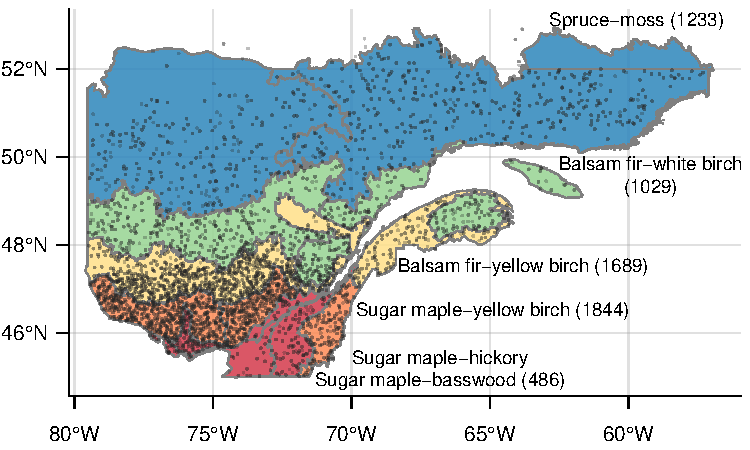
\includegraphics[width=5in,height=\textheight]{ms/figures/fig1_region.pdf}

\textbf{Figure 1.} Locations of the 6281 forest inventory plots in
meridional Québec, Canada. Colors delimit the six bioclimatic domains.
The two southernmost domains (orange) were combined in our analyses. The
number of forest plots in each domain is written in parentheses.

\pagebreak

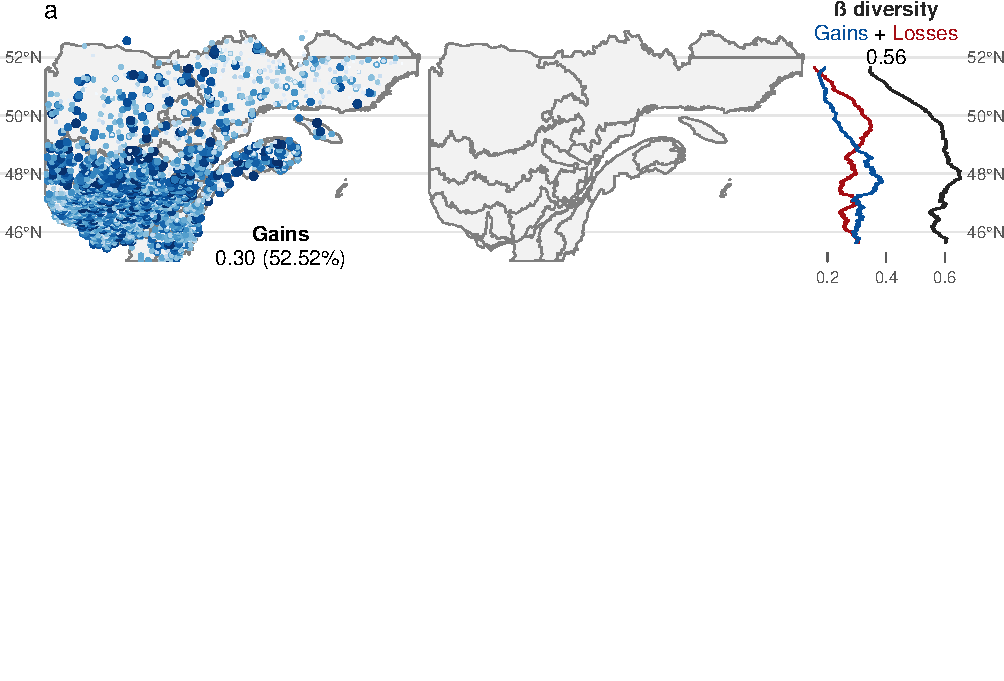
\includegraphics[width=6.7in,height=\textheight]{ms/figures/fig2_map_roll.pdf}

\textbf{Figure 2.} Maps of gains and losses in tree abundances (a) and
latitudinal trends in temporal ß diversity, decomposed into gains (blue)
and losses (red) of boreal, pioneer and temperate trees, for different
levels of disturbance (b-d). The sizes and colors of the points on the
maps are proportional to the values of interest. The latitudinal trends
in temporal ß in a-d are based on moving averages computed on each index
against latitude (window size of 500 plots in panel a and 400 plots in
panels b-d), to smooth out local-scale fluctuations and highlight
broad-scale trends.

\pagebreak

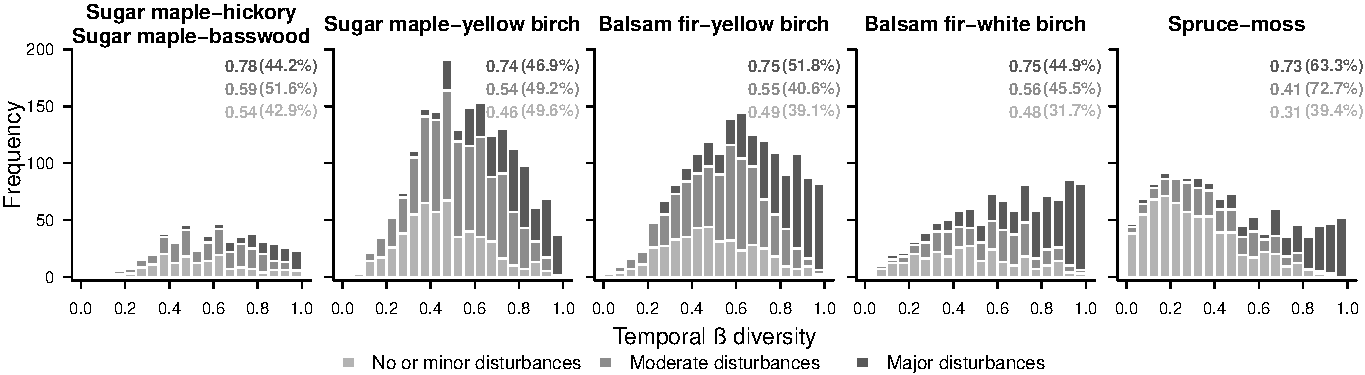
\includegraphics[width=6.7in,height=\textheight]{ms/figures/fig3_hist.pdf}

\textbf{Figure 3.} Frequency distributions of temporal ß diversity in
forests plots by bioclimatic domains. Forests of different disturbance
levels are stacked on top of each other. The values written in the
panels are the mean temporal ß diversity values followed by the
percentage of losses in parentheses. The distribution of ß diversity
values is skewed to the right for higher disturbance levels.

\pagebreak

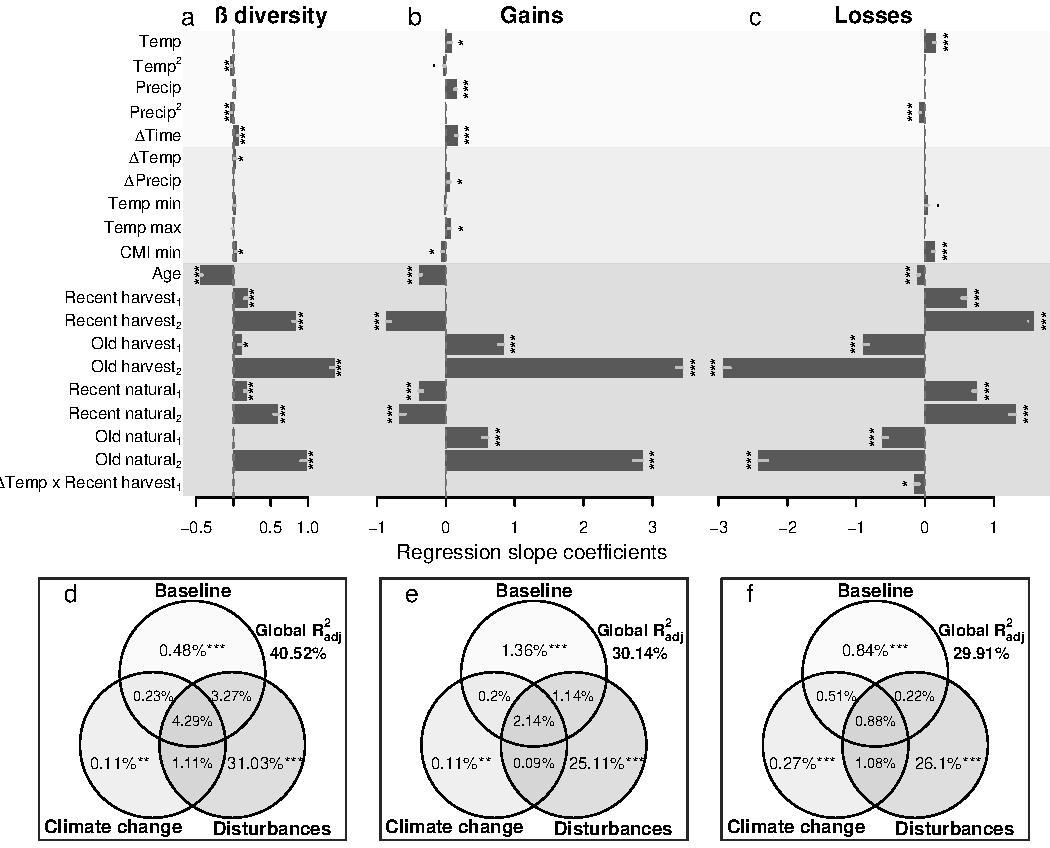
\includegraphics[width=6.6in,height=\textheight]{ms/figures/fig4_reg.pdf}

\textbf{Figure 4.}

Slope coefficients from multiple regression models for (a) temporal ß
diversity, (b) species gains and (c) species losses and the
corresponding variation partitioning diagrams (d, e, f). Error bars
represent one standard error of the slope coefficient. For the
regression models, only the selected predictors are shown. Subscripts
following disturbance predictors indicate their levels of intensity: 1
Moderate and 2 Major. In each variation partitioning, significance of
each unique fraction was tested using 9999 permutations, while shared
fractions cannot be tested. Stars indicate the level of significance of
the \emph{p}-values (* \emph{p} \textless{} 0.05; ** \emph{p}
\textless{} 0.01; *** \emph{p} \textless{} 0.001). See Table 1 for
description of the predictor variables.

\pagebreak

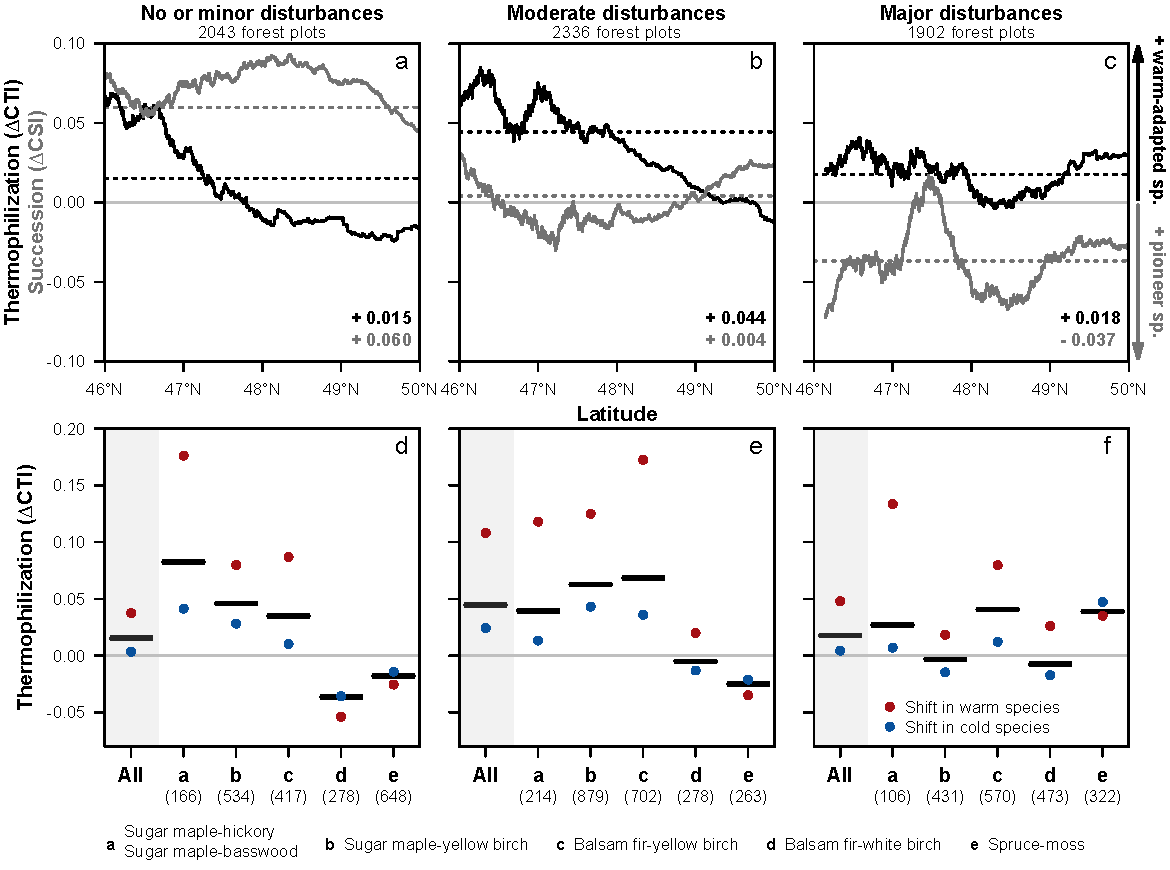
\includegraphics[width=6.6in,height=\textheight]{ms/figures/fig5_thermo.pdf}

\textbf{Figure 5.}

Thermophilization (i.e., change in community temperature index,
\(\Delta\)CTI) and successional process (i.e., change in community shade
index, \(\Delta\)CSI) of forests for different levels of disturbance. In
the upper panels (a, b, c), the latitudinal trends in \(\Delta\)CTI
(black curve) and \(\Delta\)CSI (grey curve) are based on moving
averages computed on the indices against latitude (window size of 400
plots). Positive values indicate an increase in warm-adapted species
(black) or in late-successional species (grey) over time. The dotted
lines in (a, b, c) represent the mean \(\Delta\)CTI (black) and
\(\Delta\)CSI (grey) values for different levels of disturbance. In the
lower panels (d, e, f), thermophilization of the forest plots across the
study area (All) and by bioclimatic domain. Temporal shift of the mean
(black line), left tail (red) and right tail (blue) of the distribution
of CTI, for which positive values indicate overall thermophilization,
increases of warm-adapted and decreases of cold-adapted species,
respectively.

\pagebreak

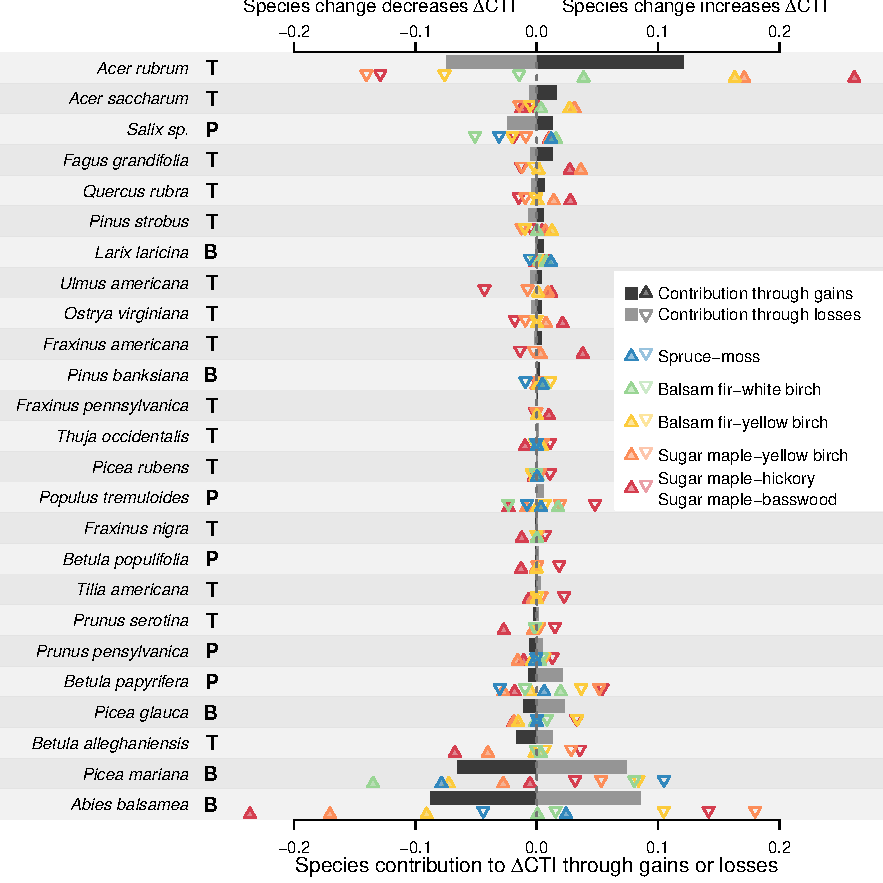
\includegraphics[width=5.8in,height=\textheight]{ms/figures/fig6_spcontrib_cti.pdf}

\textbf{Figure 6.}

Individual species contributions, through gains and losses, to
thermophilization of forest communities across the study area and for
each bioclimatic domain. The rectangles represent the mean contributions
of given species through gains (dark grey) or losses (light grey) across
the study area, while the colored triangles represent the mean
contributions of given species through gains (solid) or losses (empty)
by domain. For example, the \(\Delta\)CTI increased by an average of
0.12 for all plots where \emph{Acer rubrum} has increased in abundance
(dark grey bar), whereas the \(\Delta\)CTI also increased by an average
of 0.09 for all plots where \emph{Abies balsamea} has decreased in
abundance (light grey bar). Letters next to species names correspond to
(T)emperate, (P)ioneer and (B)oreal species. Only species that
contributed more than 0.01 in at least one domain are shown.

\end{document}
